\chapter{Installation de Ubuntu sous VM}

Un tutoriel d'installation de Ubuntu 20.04 et ROS2 est disponible en cliquant  
\href{https://insa-strasbourg-urrmc.readthedocs.io/fr/latest/index.html}{ici}.  
L'installation sur machine virtuelle suit des étapes similaires, le tutoriel ci-dessous reprend les informations de ce site internet.

\underline{Note :}Si l'objectif final est de faire de la simulation, il n'est pas recommandé d'utiliser une machine virtuelle, les performances sous VM ne permettent pas de faire tourner Gazebo convenablement.

\section{Prérequis}

\begin{itemize}
    \item Télécharger l'image ISO de Ubuntu 22.04 depuis le site officiel de Ubuntu (desktop) :  \\
    \href{https://releases.ubuntu.com/jammy/}{\url{https://releases.ubuntu.com/jammy/}}
    \item Télécharger et installer Oracle VM VirtualBox depuis le site officiel de VirtualBox :  \\
    \href{https://www.virtualbox.org/wiki/Downloads}{\url{https://www.virtualbox.org/wiki/Downloads}}
\end{itemize}

\section{Création de la machine virtuelle}

\begin{itemize}
    \item Ouvrir VirtualBox.
    \item Cliquer sur "Nouvelle" pour créer une nouvelle machine virtuelle.
    \item Donner un nom à la machine virtuelle (par exemple "Ubuntu 20.04") et sélectionner le type "Linux" et la version "Ubuntu (64 bits)".
    \item Charger l'image ISO d'Ubuntu 22.04 téléchargée précédemment.
    \item Cliquer sur "Skip Unattended Installation".
\end{itemize}

\begin{figure}[H]
    \centering
    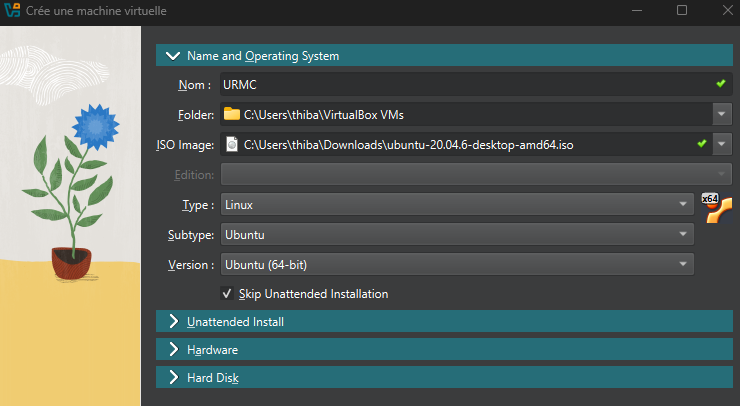
\includegraphics[width=0.8\textwidth]{Annexes/Install_Ubuntu/pictures/vm_nom_et_iso.png}
    \caption{Initialisation de la machine virtuelle}
\end{figure}

\begin{itemize}
    \item Créer un domaine d'utilisateur, avec un nom d'utilisateur (Username) et un mot de passe (Password).
    \item Définir la taille de la mémoire vive (RAM) allouée à la machine virtuelle (un minimum de 4 Go est recommandé).
\end{itemize}

\begin{figure}[H]
    \centering
    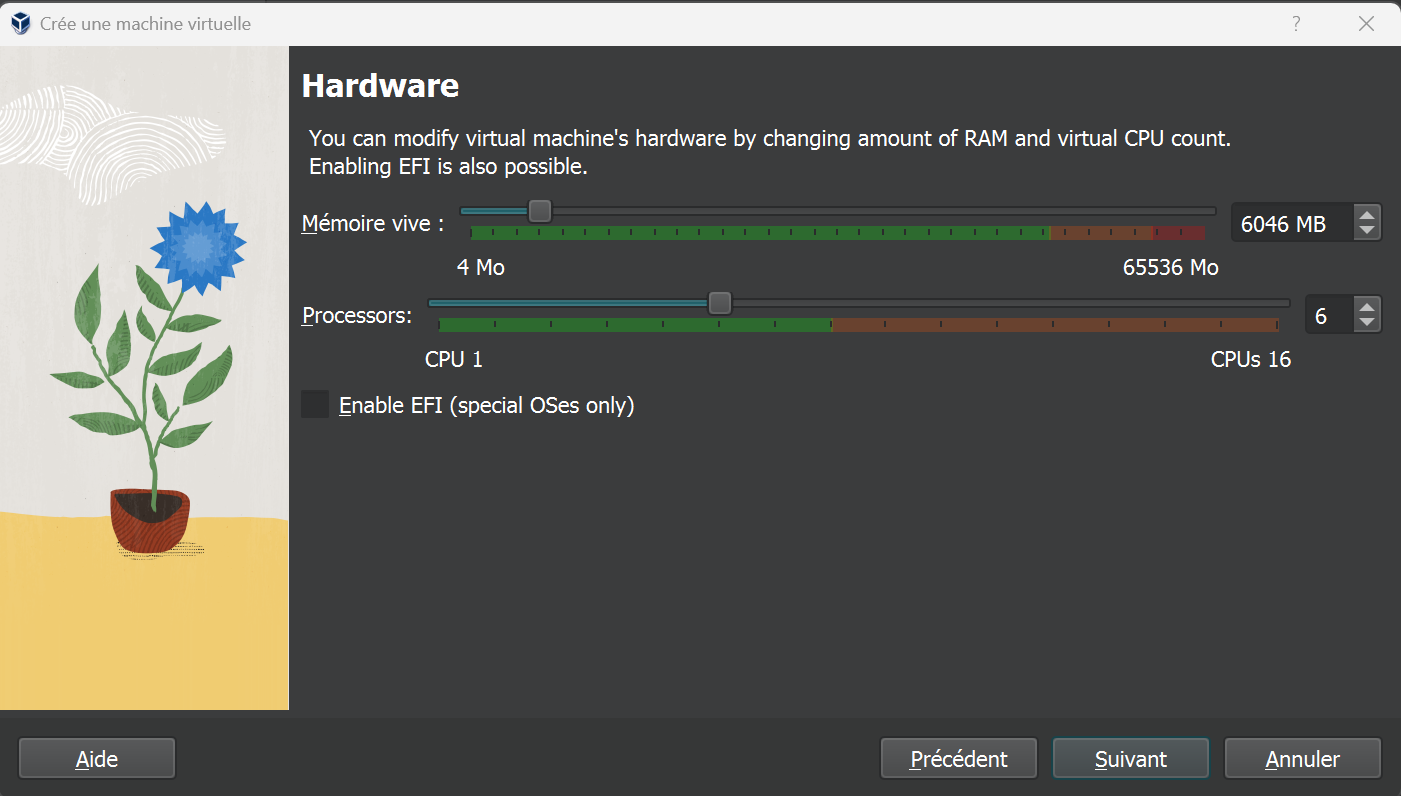
\includegraphics[width=0.8\textwidth]{Annexes/Install_Ubuntu/pictures/3Ram.png}
    \caption{Choix de la RAM pour la VM}
\end{figure}

\begin{figure}[H]
    \centering
    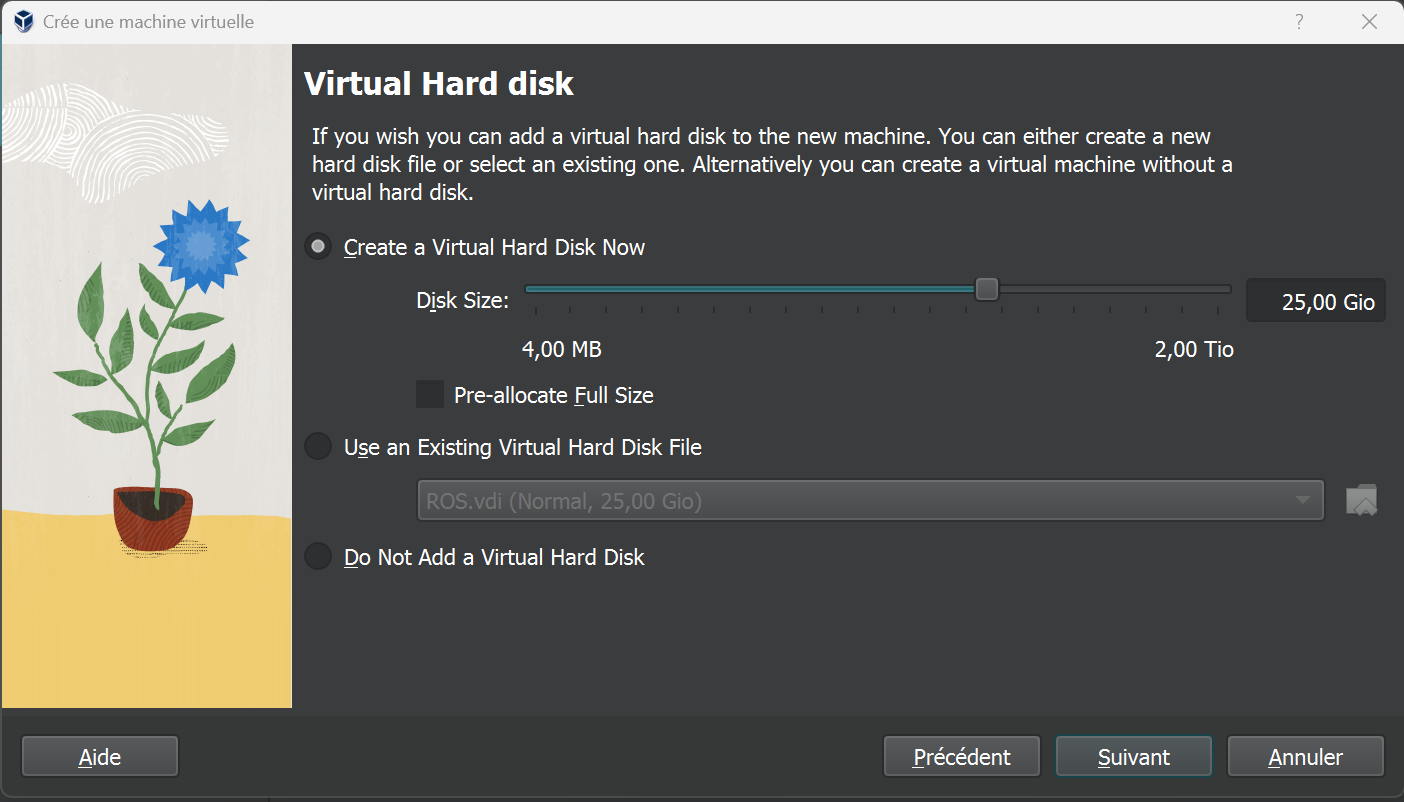
\includegraphics[width=0.8\textwidth]{Annexes/Install_Ubuntu/pictures/4Espace_disque.png}
    \caption{Choix de l'espace disque pour la VM}
\end{figure}

\begin{itemize}
    \item Cliquer sur "Créer" pour finaliser la création de la machine virtuelle.
\end{itemize}

Avant de lancer la machine virtuelle, configurer quelques paramètres supplémentaires :  
Sélectionner la machine virtuelle, appuyer sur "Configuration" et aller dans l'onglet "Expert" en haut à gauche, puis "Affichage".  
Activer, si l'ordinateur le permet, l'accélération graphique et augmenter la mémoire vidéo.  
Cela améliore les performances graphiques de la machine virtuelle. Cependant, selon la version de Gazebo utilisée, cela peut complètement empêcher le logiciel de fonctionner.

\newpage

\begin{figure}[H]
    \centering
    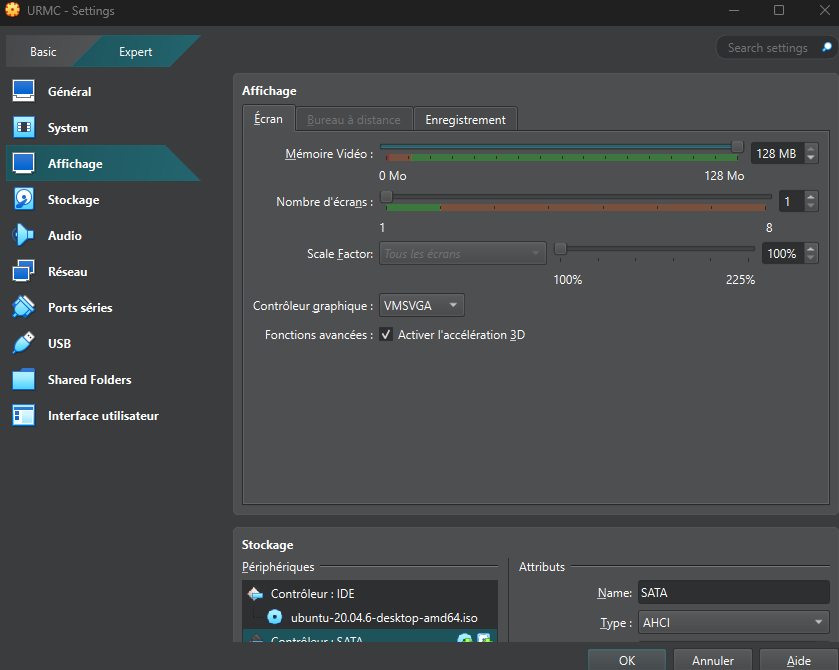
\includegraphics[width=0.8\textwidth]{Annexes/Install_Ubuntu/pictures/acc_graph.png}
    \caption{Accélération graphique}
\end{figure}

\section{Configuration de la machine virtuelle}

\begin{enumerate}
    \item Sélectionner la machine virtuelle dans la liste et cliquer sur "Démarrer".
    \item Suivre les étapes d'installation d'Ubuntu, en choisissant les paramètres appropriés.
    \item Une fois l'installation terminée, se connecter avec les identifiants créés précédemment.
\end{enumerate}

\section{Configuration du clavier et de la résolution}

\subsection*{Modification du clavier}

\begin{itemize}
    \item Aller dans les paramètres système, dans la section "Langues et région".
    \item Cliquer sur "Gérer les langues installées" et ajouter le français comme langue.
    \item Sélectionner le français comme langue par défaut.
\end{itemize}

\subsection*{Modification de la résolution}

\begin{itemize}
    \item Dans les paramètres de la machine virtuelle, aller dans l'onglet "Écran".
    \item Ajuster la "Définition" en fonction de la résolution de l'écran.
\end{itemize}